\documentclass{beamer}
\usepackage{pgfpages}
\usepackage{newtxtext,newtxmath} %time new roman
%\setbeameroption{show notes}
%\setbeameroption{show notes on second screen=right}
\usetheme{Warsaw}
\usepackage[french]{babel}

\usepackage{tikz}
\pgfdeclareimage[height=0.5cm]{le-logo}{}
%\setbeamertemplate{footline}[frame number]
%Set number slide 

\usepackage[backend=biber]{biblatex}
%\usepackage[backend=biber, style=chem-acs]{biblatex}
\addbibresource{presentation.bib} 
\bibliography{Skin Cancer Detection}
\setbeamertemplate{bibliography item}[triangle]

\usepackage{multirow}% row fusion
\usepackage{array} % column fusion
\usepackage{xfrac} % small fractions
\usepackage{adjustbox}
\usepackage{listings}
\usepackage{color}
\definecolor{gray}{rgb}{0.4,0.4,0.4}
\definecolor{darkblue}{rgb}{0.0,0.0,0.6}
\definecolor{cyan}{rgb}{0.0,0.6,0.6}
 \titlegraphic{\vspace{-1cm}
      
\includegraphics[width=2.5cm]{images/paris8_1}\hspace*{4.75cm}~%
      \hfill
      
\includegraphics[width=2.5cm]{images/logo}
}
\setbeamertemplate{frametitle}{\nointerlineskip  
    \begin{beamercolorbox}[wd=\paperwidth,ht=2.75ex,dp=1.375ex]{frametitle}
        \hspace*{2ex}\insertframetitle \hfill {\small\insertframenumber/\inserttotalframenumber} \hspace*{1ex}%
    \end{beamercolorbox}}

\usecolortheme{wolverine}
\setbeameroption{hide notes} % Only slides


%%%%%%%%%%%%%%%%%%%%%%%%%%%
\title[Body Tumor Detection Using Convolutional Neural Network] 
{Tumor Detection Using Convolutional Neural Network}
%\subtitle {ne compléter que si l'article possède un sous-titre}
\author[Komlan Dantodji] 
{Komlan Jean-Marie DANTODJI}

\institute[]
{
  Etudiant en M1 Big Data
  \and
  Université Paris 8}
\date{March 7, 2020}


\begin{document}
\begin{frame}
  \titlepage
\end{frame}

\begin{frame}{Summary}
  \tableofcontents
\end{frame}

\section{Introduction}
\begin{frame}{Tumor in body}
\begin{figure}[H]
    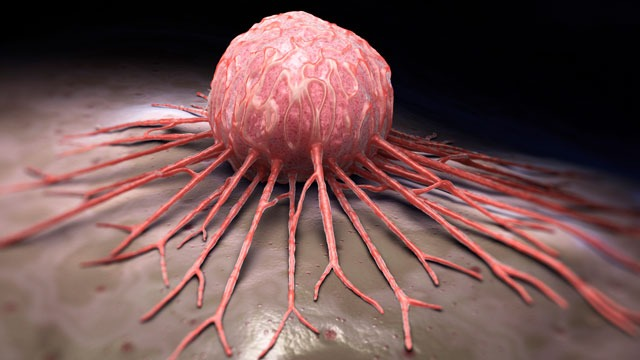
\includegraphics[width=8cm,height=4cm]{images/tumor.jpg}
    \caption{ Body Tumor: From Google}
    \label{fig:L1}
\end{figure}
\end{frame}

\section{Issue}
\begin{frame}{Issue}
\begin{itemize}
		\item Find a way to diagnostic tumors cells from an image 
		\item Extract features from the image
		\item Apply Convolutional Neuronal Network to layers 
\end{itemize}
\end{frame} 


\section{Input image and Dataset}
\begin{frame}{Input image and Dataset}
\begin{itemize}
		\item Image of patient's body
		\item Dataset of images from Database
\end{itemize}
\end{frame} 
%\begin{frame}{Skin Cancer}
%\end{frame} 
\section{Differents step of detecting tumor in image} 
\begin{frame}{Chart of steps}
\begin{figure}[H]
    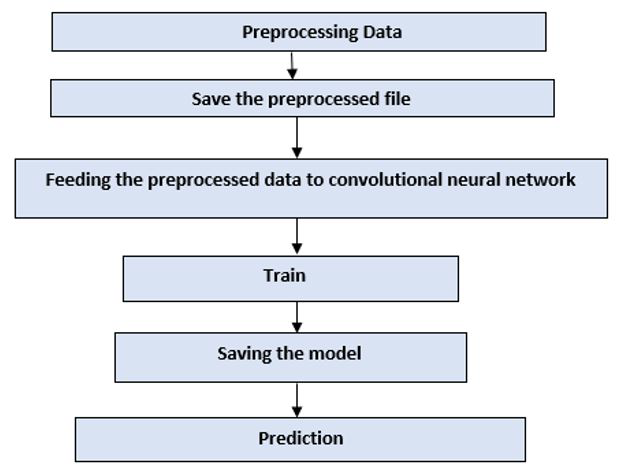
\includegraphics[width=8cm,height=4.5cm]{images/steps.png}
    \caption{[1] Chart display steps of the model CNN, page 255}
    \label{fig:L1}
\end{figure}
\end{frame} 
\begin{frame}{Step 1: Preprocessing Data}
\begin{itemize}
		\item Convert all images to the gray-scale
		\item Resize images to reduce time of processing
\end{itemize}
\end{frame} 

\begin{frame}{Step 2: Save the preprocessed file}
\begin{itemize}
		\item  Binary labels: benign and malignant
		\item Classify each image of dataset to his class
\end{itemize}
\end{frame} 

\begin{frame}{Step 3: Feeding the preprocessed data to CNN 1/3}
\begin{figure}[H]
    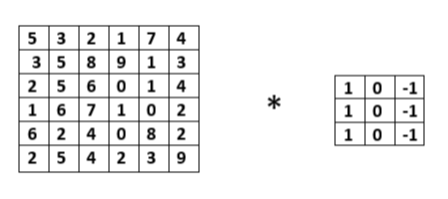
\includegraphics[width=7cm,height=3cm]{images/convolution.png}
    \caption{[1] Gray-scale Image 6x6 and the 3x3 filter, page 256}
    \label{fig:L1}
\end{figure}
$$ \sum_{i=0}^{m-1}\sum_{i=0}^{m-1} X_{(n-i)(n-j)}Y_{(i+1)(j+1)}    (1)$$
\end{frame} 

\begin{frame}{Step 3: Result of Pooling 2/3}
We get the result as follow:
\begin{figure}[H]
    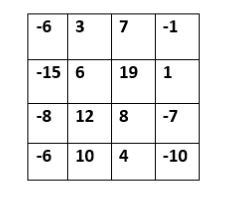
\includegraphics[width=7cm,height=4cm]{images/pooling.png}
    \caption{[1] 4x4 image after applying 3x3 filter to the gray-scale image, page 257}
    \label{fig:L1}
\end{figure}
\end{frame} 

\begin{frame}{Step 3: Max Pooling 3/3}
Extract more features
\begin{figure}[H]
    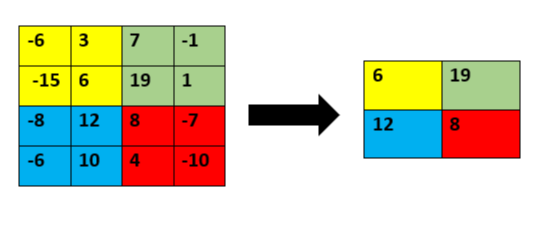
\includegraphics[width=7cm,height=3cm]{images/maxpooling.png}
    \caption{[1] Result after applying max pooling, page 257}
    \label{fig:L1}
\end{figure}
\end{frame} 

\begin{frame}{Steps 4 and 5: Train and save the model}
\begin{itemize}
		\item  Train the model 200 times of epoch
		\item Save the model 
\end{itemize}
\end{frame} 




\section{Conclusion}
\begin{frame}{Conclusion}
\begin{itemize}
		\item Helps dermatologist to dignostisic early skin cancer 
		\item Hight accuracy with the model CNN
\end{itemize}
\end{frame}

\begin{frame}{Reference}
\par [1] Hasan, Samia Islam, Surajit Das Barman, Skin Cancer Detection Using Convolutional Neural Network,Mahamudul from the 2019 5th International Conference in April 2019, pages 254-258
\end{frame}

\begin{frame}
  \begin{block}{}
  \centering
  Thank you for your attention...
  \end{block}
\end{frame}
\end{document}
